%!TEX root = ../thesis.tex

\chapter{Grundlagen}

Im nachfolgenden werden Grundlagen erläutert, die als Basis des Projects dienen, so wie zum Verständnis des Kapitels `Frameworks' erforderlich sind.


\section{Cross Device Entwicklung}
Lorem ipsum dolor sit amet, consetetur sadipscing elitr, sed diam nonumy eirmod tempor invidunt ut labore et dolore magna aliquyam erat, sed diam voluptua. At vero eos et accusam et justo duo dolores et ea rebum. Stet clita kasd gubergren, no sea takimata sanctus est Lorem ipsum dolor sit amet. Lorem ipsum dolor sit amet, consetetur sadipscing elitr, sed diam nonumy eirmod tempor invidunt ut labore et dolore magna aliquyam erat, sed diam voluptua. At vero eos et accusam et justo duo dolores et ea rebum. Stet clita kasd gubergren, no sea takimata sanctus est Lorem ipsum dolor sit amet.

\section{Cross Platform Entwicklung}
Lorem ipsum dolor sit amet, consetetur sadipscing elitr, sed diam nonumy eirmod tempor invidunt ut labore et dolore magna aliquyam erat, sed diam voluptua. At vero eos et accusam et justo duo dolores et ea rebum. Stet clita kasd gubergren, no sea takimata sanctus est Lorem ipsum dolor sit amet. Lorem ipsum dolor sit amet, consetetur sadipscing elitr, sed diam nonumy eirmod tempor invidunt ut labore et dolore magna aliquyam erat, sed diam voluptua. At vero eos et accusam et justo duo dolores et ea rebum. Stet clita kasd gubergren, no sea takimata sanctus est Lorem ipsum dolor sit amet.

\section{Web Components}

\subsection{Einführung}

Moderne Webanwendungen sind heutzutage meist nicht nur in ihrem Design komplex, komplexität lässt sich auch meist nicht in der Entwicklung
vermeiden. Dieses Problem wird noch brisanter, wenn eine Applikation über einen langen Zeitraum hinweg,
womöglich von verschiedenen Entwicklerteams, entwickelt und betreut wird. Schaut man sich den DOM von Patrioten des Internets wie Facebook oder Amazon an,
wird schnell klar, dass deren Domstruktur durch Inflationäre Nutzung von DIV und SPAN Tags schnell zu Unübersicht führt,
da die Palette an HTML5 Semantic Tags nicht ausreicht, um die Funktionalitäts Vielfalt einer modernen Webanwendung abzudecken.
Statt aussagekräftige Tags zu verwenden, muss man sich mit Klassen und IDs behelfen, um Elemente überhaupt voneinander unterscheiden zu können.
\cite{sitepoint-introduction-to-webcomponents}

\subsection{Komponenten in der Softwarentwicklung}
Lorem ipsum dolor sit amet, consetetur sadipscing elitr, sed diam nonumy eirmod tempor invidunt ut labore et dolore magna aliquyam erat, sed diam voluptua. At vero eos et accusam et justo duo dolores et ea rebum. Stet clita kasd gubergren, no sea takimata sanctus est Lorem ipsum dolor sit amet. Lorem ipsum dolor sit amet, consetetur sadipscing elitr, sed diam nonumy eirmod tempor invidunt ut labore et dolore magna aliquyam erat, sed diam voluptua. At vero eos et accusam et justo duo dolores et ea rebum. Stet clita kasd gubergren, no sea takimata sanctus est Lorem ipsum dolor sit amet.



\subsection{Web Components}

``Web Components are an emerging set of standards from the W3C to describe a way to create encapsulated,
reusable blocks of UI presentation and behavior entirely with client side languages- HTML, JavaScript and CSS.''
\cite[42]{Web-Component-Architecture}
\vspace{1cm}

Standards des W3C beschreiben diverse Wege wie entkoppelte wiederverwendbare UI Elemente,
in Kombination von HTML, JavaScript und CSS, so genannte Web Components, geschaffen werden können.
Der Begriff Web Components beinhaltet somit eine Sammlung von Standards,
welche die bereits genannte Problematik der fehlenden HTML Semantic mit bestehenden Webtechnologien lösen soll.
Web Components sollen wie wiederverwendbare Web Widgets mit klar definierten Schnittstellen funktionieren.
Dabei sollen sie im Browser implementiert sein und ohne externe Bibliotheken nutzbar sein.
Bestehende Web Komponenten sollen ohne Code funktionsfähig sein. Lediglich durch das Einfügen der Komponente in das Markup,
soll bereits Funktionalität zur Verfügung stehen.
\cite[42]{Web-Component-Architecture}

\subsubsection{Features}
Lorem ipsum dolor sit amet, consetetur sadipscing elitr, sed diam nonumy eirmod tempor invidunt ut labore et dolore magna aliquyam erat, sed diam voluptua. At vero eos et accusam et justo duo dolores et ea rebum. Stet clita kasd gubergren, no sea takimata sanctus est Lorem ipsum dolor sit amet. Lorem ipsum dolor sit amet, consetetur sadipscing elitr, sed diam nonumy eirmod tempor invidunt ut labore et dolore magna aliquyam erat, sed diam voluptua. At vero eos et accusam et justo duo dolores et ea rebum. Stet clita kasd gubergren, no sea takimata sanctus est Lorem ipsum dolor sit amet.

\subsubsection{Vorteile}
Lorem ipsum dolor sit amet, consetetur sadipscing elitr, sed diam nonumy eirmod tempor invidunt ut labore et dolore magna aliquyam erat, sed diam voluptua. At vero eos et accusam et justo duo dolores et ea rebum. Stet clita kasd gubergren, no sea takimata sanctus est Lorem ipsum dolor sit amet. Lorem ipsum dolor sit amet, consetetur sadipscing elitr, sed diam nonumy eirmod tempor invidunt ut labore et dolore magna aliquyam erat, sed diam voluptua. At vero eos et accusam et justo duo dolores et ea rebum. Stet clita kasd gubergren, no sea takimata sanctus est Lorem ipsum dolor sit amet.

\subsubsection{Polyfills}
Lorem ipsum dolor sit amet, consetetur sadipscing elitr, sed diam nonumy eirmod tempor invidunt ut labore et dolore magna aliquyam erat, sed diam voluptua. At vero eos et accusam et justo duo dolores et ea rebum. Stet clita kasd gubergren, no sea takimata sanctus est Lorem ipsum dolor sit amet. Lorem ipsum dolor sit amet, consetetur sadipscing elitr, sed diam nonumy eirmod tempor invidunt ut labore et dolore magna aliquyam erat, sed diam voluptua. At vero eos et accusam et justo duo dolores et ea rebum. Stet clita kasd gubergren, no sea takimata sanctus est Lorem ipsum dolor sit amet.


\section{Typescript}

\subsection{Entwicklung von Javascript}

\begin{figure}[ht]
 \centering
 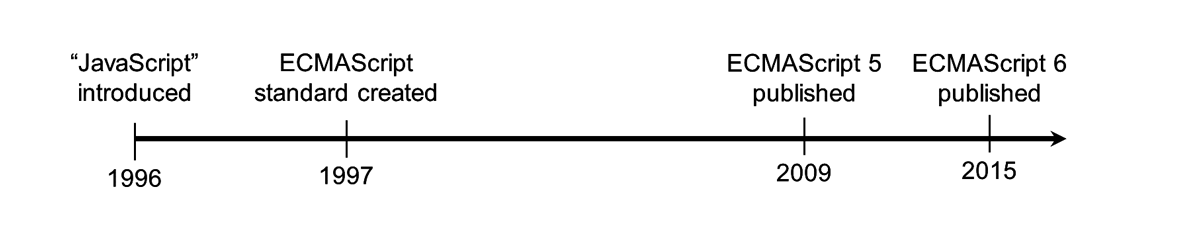
\includegraphics[width=\linewidth]{kapitel2/javascript-timeline.png}
 \caption{History of Javascript}\cite[28]{EssentialTS}
\end{figure}

Javascript wurde erstmals 1996 von Brendan Eich in einer Implementierung des Netscape Navigator Browsers eingeführt,
worauf weitere Browser die Syntax und APIs ähnlich, jedoch nicht identisch nach implementierten.
Daraufhin veröffentlichte die ECMA International einen Standard, welcher die Spezifikationen der neuen Sprache
definieren sollte. Dieser trägt den namen ECMAScript und ist der offizielle und bekannteste Standard der
Sprache. ActionScript von Macromedia und JScript von Microsoft sind weitere Implementierungen der Browsersprache,
die nicht dem ECMA Standard entsprechen, jedoch darauf aufbauen.

1997 wurde die erste Versionen des nun standardisiertem ECMAScript veröffentlicht. Ein Jahr später erschien bereits ECMAScript2,
allerdings beinhaltete dieses Update nur kleine Änderungen um einem parallel entstandenen ISO Standard von JavaScript zu implementieren.
Die nächste große Neuerung kam 1999 mit ECMAScript3, in welcher einige innovative Features implementiert wurden.
``[...]regular expressions, better string handling, new control statements, try/catch exception handling, tighter definition of errors, formatting for numeric output and other enhancements.''\cite{js-vs-es}.

Das nächste Update ECMAScript4 war 2008 geplant, zunächst als Prototyp entwickelt,
jedoch noch vor dem Release, aufgrund eines rückschritttigem Featureset wieder aufgegeben.
Zur selben Zeit entwickelte sich Ajax und damit eine völlig neue Art von dynamsichen Webapplikationen,
basierend auf JavaScript.

2009 erschien ECMAScript5, mit vollem Support in allen verbreiteten Webbrowsern, abgesehen vom Internet Explorer.
Neue Features waren unter anderem JSON support und klassische Array Funktionen wie map und forEach.
Durch die Entfernung einiger Features wurde JavaScript in der neuen Version sauberer und stabiler.

ECMAScript6 sollte bereits 2013 veröffentlicht werden, der offizielle Releasetermin wurde
dann allerdings bis in den Juni 2015 verschoben und ist bis heute noch nicht ausreichend in allen Browsern implementiert.
\cite{js-vs-es}

\subsection{Allgemein}

Typescript ist eine von Microsoft entwickelte Programmiersprache.
Die Sprache ist ein Superset von ES6, d.h. sie implementiert den JavaScript Standard und ergänzt diesen
durch zusätzliche Features, wie der statischen Typisierung.
Typescript will ausgereifter, robuster und speziell in großen Projekten eine solidere Alternative sein. \cite[28]{EssentialTS}
Zusammen mit ES6 erhalten wir gegenüber ES5 folgende Features:

\begin{figure}[ht]
 \centering
 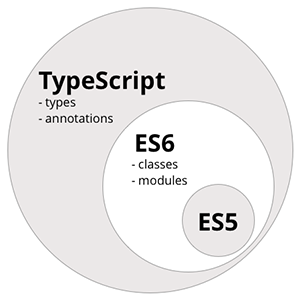
\includegraphics[width=0.4\linewidth]{kapitel2/typescript----es5-es6-typescript-circle-diagram.png}
 \caption{Language Relationship}\cite[152]{ng-Book-2}
\end{figure}


\subsubsection{statische Typisierung}

Die wohl größte Erungenschaft der Sprache ist das statische Typsystem.
Typenfehler können in Typescript bereits zum Zeitpunkt
der Kompilierung bzw. Transpilierung erkannt werden und treten nicht erst zur Laufzeit im Browser auf.
Zudem wird Code in einer Typescript unterstützenden IDE dank Autovervollständigung
leichter zu schreiben und aussagekräftiger zu lesen.\cite[156]{ng-Book-2}

\subsubsection{Klassen}

Mit ES6 Klassen wurde eine neue Syntax für das prototypische Vererbungsmodell von Javascript entwickelt.
Dabei handelt es sich nicht um die Einführung eines neuen OOP-Modells, sondern lediglich um eine vereinfachte Syntax für Objekte und deren Schnitstellen,
so wie die Realisierung von Abstraktionen, wie man sie aus anderen Objektorientierten sprachen wie C++, Swift oder Java bereits kennt.\cite{js-Klassen}

\lstinputlisting[language=Java,label=code,caption=Klassen in ES6]{kapitel2/class.js}

\subsubsection{Module}

In ES5 gab es keinen Standard um Funktionen und Variablen in Namensräumen zu organisieren, oder dynamisch Code zu laden.
Mit ES6 wurde das fehlende Feature durch exportieren und importieren von Modulen ergänzt. Dadurch wird es sehr bequem Programmcode zu organisieren und zu laden.
Jedes ES6 Modul wird in einer eigenen Datei gespeichert. Variablen und Funktionen sind von außerhalb nicht sichtbar, es sei denn sie werden explizit exportiert.
Mittels Export lassen sich also Schnittstellen für ein Modul definieren, welche mittels des Keywords Import importiert und verwendet werden können.
In Typescript lassen sich ganze Klassendefinitionen exportieren.
Dabei ist es möglich Instanzfunktionen und Instanzvariablen mit dem Keyword private vor dem äußeren Zugriff zu verstecken.
Public Funktionen sind dann wie man es aus anderen OO-Sprachen kennt, auch von außen nutzbar.

\lstinputlisting[language=Java,label=code,caption=Export und Import von Modulen in ES6]{kapitel2/module.js}

\subsection{Transpilierung}

Typescript so wie ES6 bieten Entwicklern also eine ganze Reihe von Neuerungen gegenüber den Vorgängerversionen.
Spannende Features bringen jedoch wenig, wenn sie im Standard zwar spezifiziert wurden,
allerdings noch in sehr wenigen Browsern vollständig implementiert sind.
Um TS oder ES6 Code also überhaupt in Produktion zu nutzen, sollte er auf den ES5 oder ES3
Standard herunter transpiliert werden.
Ein Transpiler ist ein Compiler, welcher Sourcecode nicht in Maschinencode, sondern ebenfalls in Sourcecode,
allerdings einer anderen Sprache oder Version der Sprache wandelt.\cite{Introduction-to-the-Typescript-Transpiler}
In der nachfolgenden Abbildung ist zu sehen, wie Typescript Code in funktionsfähigen ES5 Code transpiliert wird.

\begin{figure}[ht]
 \centering
 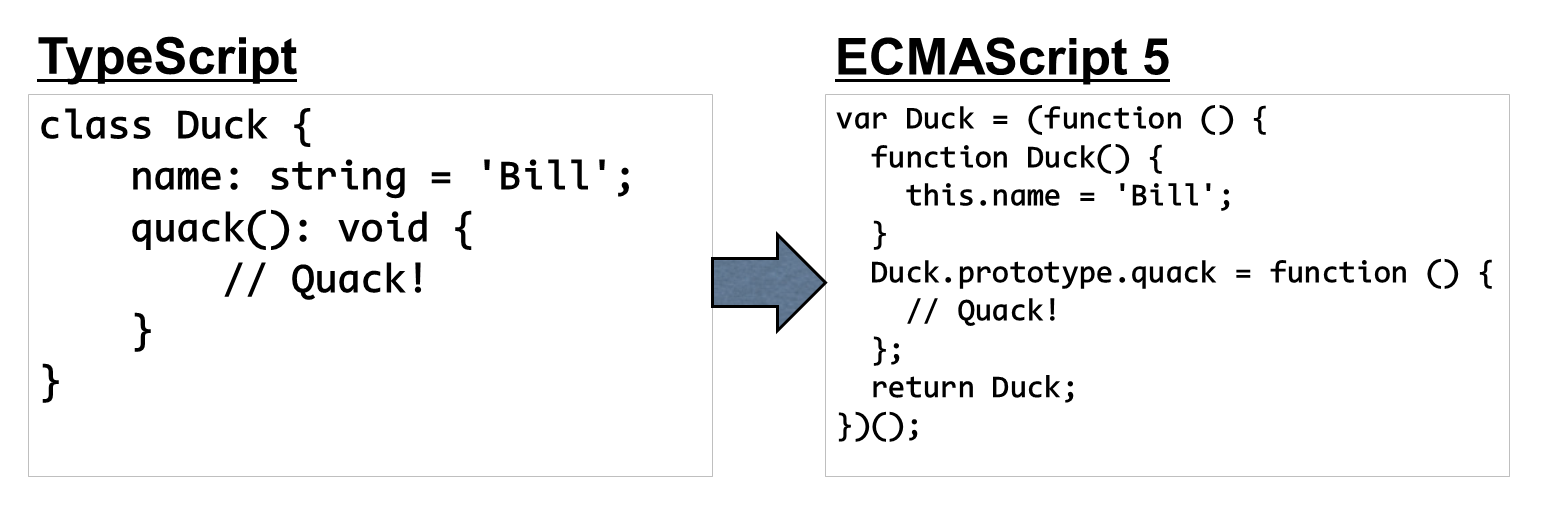
\includegraphics[width=0.8\linewidth]{kapitel2/Introduction-transpiler.png}
 \caption{Transpilierung}\cite[27]{ng-Book-2}
\end{figure}
